\documentclass{article}
\usepackage{graphicx} % Required for inserting images

\title{Homework Template}
\author{Riccardo Zucchelli 1984963}
\date{October 2024}

\begin{document}

\maketitle

\section{Introduction to Frequency Analysis}
In cryptography, \emph{frequency analysis} is a way to organize letters with their frequency. It's based on the fact that, given a certain language, it is known that each letter appears with a certain frequency on a given text. This can be very useful to break cipher based on the alphabetic substitutions. As an example, the phrase \emph{ETAOIN SHRDLU} represents the 12 most used letters in the English language.

As previously mentioned, we'll be working with a substitution cipher, in which each plain text letter is replaced by another, following a specific substitution pattern (which will be also the secret key). Given the fact that every letter will be always replaced with the same one, we can use the frequency analysis attack, comparing our findings to the one for the English language.

\begin{figure}[h]
    \centering
    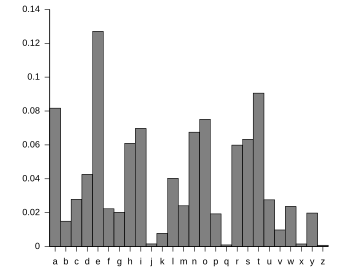
\includegraphics[width=0.8\linewidth]{image.png}
    \caption{The typical distribution in the English language}
    \label{fig:english}
\end{figure}

\section{The ciphertext, how can we attack it}

The ciphertext we'll be dealing with is the following:

PIFFMKMQI'YRKJKPQMKDJ RKJKPXAKZQXVRKNGJMXZ'KXZKTHRKVTYRRTKAQZZJKPRKJKPXAKDJZKVQDRKFJMKMQIKAQTKDIFKQZKMQ'KSJORKMQIKPXAKFXVAYJORK XO XZ'KMQIYKOJZKJGGKQLRYKTHRKNGJORKVXZAXZ'

We can plot our findings in a graph
\begin{figure}[h]
    \centering
    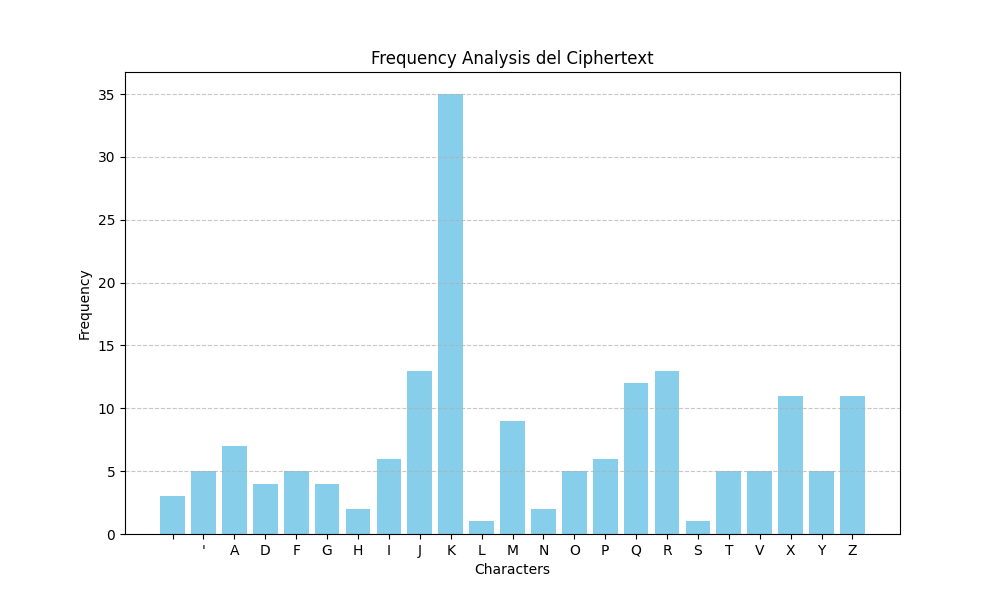
\includegraphics[width=0.8\linewidth]{frequency.png}
    \caption{The frequency analysis on the cyphertext}
\end{figure}

With these results we can already do some very basic hypotheses on the key. We can really see that the most frequent letter, that appears in 20\% of the ciphertext, is K. Given that there are also spaces in the text, but they aren't aligned with any real word, we can consider the fact that our substitutution alphabet includes the space as a character, and that the K is in reality a space. This excludes the \emph{Ceasar's Cypher}, a particular mono-alphabetic substitution cipher that replaces a letter with a different one at a fixed number of places, since we can't consider the ASCII table as the strides would be too long. 
Substituting the K with the space character we can continue our analysis

\texttt{PIFFM MQI'YR J PQM DJ\_R J PXA ZQXVR NGJMXZ' XZ THR VTYRRT AQZZJ PR J PXA DJZ VQDR FJM MQI AQT DIF QZ MQ' SJOR MQI PXA FXVAYJOR \_XO\_XZ' MQIY OJZ JGG QLRY THR NGJOR VXZAXZ'}

We'll continue by enumerating letters, ordering them by their frequencies:
\begin{enumerate}
    \item K which we already hypothesized on being the space character
    \item J/R which have the same number of appearances could be e, a or t
    \item Q which given our frequency analysis could be an o, or a t
    \item X could be i or a t
\end{enumerate}

Given the ciphertext, we can see how the J character, which appears 13 times throughout the text, is usually a single letter. In the English language, usually, this appears if it's the a character, and so we'll try substituting J with it. At this point we should try with substituting R with e, being the most frequent character.
Another clue that we can derive from this is by analyzing the bigrams that appear in the text. We'll see that the most frequent ones are XZ, MQ, QI (being MQI a frequent trigram in itself and usually a single word, which could correspond to "you") and JO (having JOR as a frequent trigram. Using the JO bigram, we can derive that the O is a n. With already decrypting 3 letters, we can start and see if we can assume some word. We have you'YR, which can be only be decrypted with "you're", oLer, which is "over". VTreeT is a word in which the second and the last letters match, so it makes "street" the only word possible.

We can stop here, as we decrypted a good chunk of the alphabet and we got:
\texttt{PuFFy you're a Poy Da\_e a PXA ZoXse NGayXZ' XZ tHe street AoZZa Pe a PXA DaZ soDe Fay you Aot DuF oZ yo' SaOe you PXA FXsAraOe \_XO\_XZ' your OaZ aGG over tHe NGaOe sXZAXZ'}
Which we can find perfectly correlates with the famous Queen song \emph{We will rock you}.

\section{The result}
We now have completely cracked the code, using frequency analysis techniques on single words, bigrams, trigrams and whole words by themselves, thanks to online tools provided for free on 
\begin{itemize}
    \item \texttt{https://wilsoa.github.io/gallery/frequency\_analysis.html}
    \item \texttt{https://www.wordhippo.com/what-is/word-finder-unscrambler.html}
\end{itemize}

Which all made possible to decrypt the ciphertext with:
\begin{center}
\emph{Buddy you're a boy make a big noise
Playin' in the street gonna be a big man some day
You got mud on yo' face
You big disgrace
Kickin' your can all over the place
Singin'}
\end{center}

\end{document}
